\section{第5章\quad 微波网络理论与分析}
\begin{frame}{第5章\quad 微波网络基础}
    电磁场理论和网络理论代表着不同的两个方面:场是网络的内部原因,而网络则是场的外部表现。
\end{frame}

\subsection{微波网络概念及等效关系}
\begin{frame}{微波网络概念及等效关系}
    微波网络由分布参数电路和集总参数网络组合而成。分布参数电路由组成微波电路或系统的规则导行系统等效而成,集总参数网络则由微波电路或系统中的不连续性等效而成。
    应用这种等效关系,许多微波问题,在电磁场理论分析基础上,或者在实验的基础上,便可以应用传输线理论和低频网络理论来处理。
\end{frame}
\begin{frame}{微波网络概念及等效关系}
    考虑一个不均匀区域:一个具有理想导体壁的$n$口波导结构,除了$n$个端口外,其余部分与外界没有场的联系,如图所示。若作一封闭面$S$将其包围起来,并将$S$和各波导
    垂直相交的截面选座参考面,且用$T_1,T_2,\cdots,T_n$表示,则其结构内的电磁场应满足$Maxwell$方程组。\\
    最基本的方法:求解电磁场方程。但是在整个电路范围内求解电磁场方程非常复杂,难以工程应用。
    \begin{columns}
        \begin{column}{0.6\linewidth}
            \textbf{微波网络方法}:将射频电路分解为传输线和不连续性的组合,然后对传输线和不连续性分别建模。\\
            网络方法的思想:化繁为简、各个击破,把复杂的三维电磁场问题变为一维电路问题。
        \end{column}
        \begin{column}{0.4\linewidth}
            \begin{figure}
                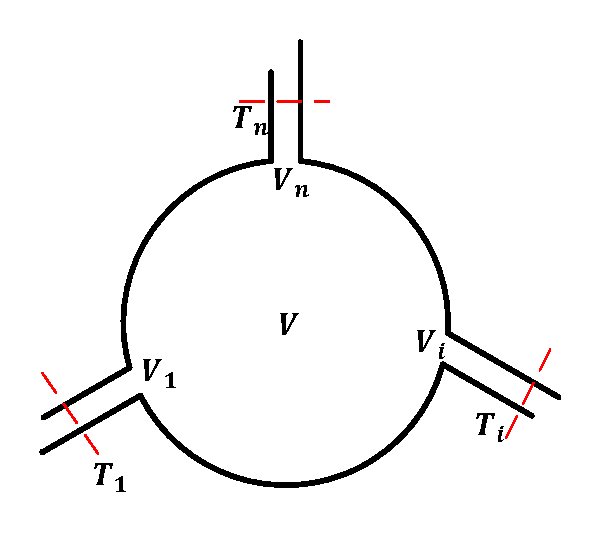
\includegraphics[width=4.5cm]{Cha5//fig5-1.pdf}
            \end{figure}
        \end{column}
    \end{columns}
\end{frame}

\begin{frame}{微波网络概念及等效关系}
    \begin{itemize}
        \item 传输线建模\\
              把传输线等效为双线,用特征参数表征。单模传输线等效为一条双线,$n$模传输线等效为n条传输线。
        \item 不连续性建模\\
              可以采用等效电路模型,也可以采用网络矩阵表征。
        \item 通过建模,射频电路等效为由传输线和不连续性网络构成的电路。射频电路就可以采用电路理论分析和设计,“场方法”转化为“路方法”。
    \end{itemize}
\end{frame}

\begin{frame}{微波网络概念及等效关系}
    当波从一传输线入射到一不连续性区域时,一部分反射会传输线,其余部分通过不连续性区域传输到其他传输线,同时在不连续性区域激发出高次模,
    这些高次模在传输线中为截止波,所以很快衰减掉。这样在不连续性附近就形成了一个能量存储区,相当于电抗元件。\\
    \hspace*{\fill}\\
    以网络的观点,不连续性区域可以看作连接传输线的网络。在传输线上适当位置选取参考面$T$,不连续性区域就可以等效为多端口网络。
    \begin{figure}
        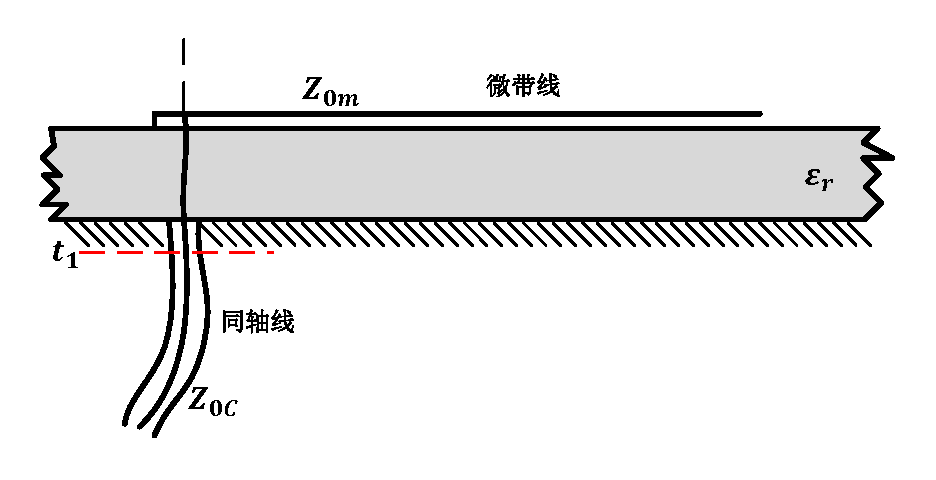
\includegraphics[width=5cm]{Cha5//fig5-2.pdf}
        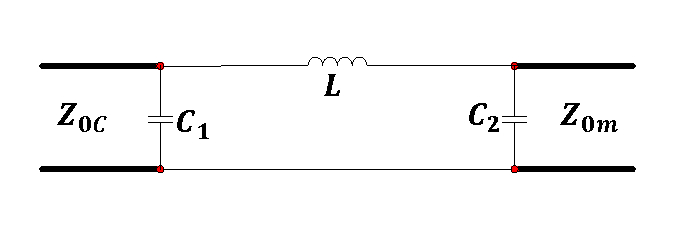
\includegraphics[width=6.5cm]{Cha5//fig5-3.pdf}
    \end{figure}
\end{frame}

\begin{frame}{微波网络概念及等效关系}
    \begin{enumerate}
        \item 微波传输线等效为双线
              \begin{itemize}
                  \item 等效阻抗:等效电压和等效电流之比
                        $$Z(z)=\frac{V(z)}{I(z)}$$
                  \item 归一化等效阻抗
                        $$z=\frac{Z(z)}{Z_0}=\frac{V(z)/\sqrt{Z_0}}{I(z)\sqrt{Z_0}}=\frac{1+\Gamma(z)}{1-\Gamma(z)}$$
                        归一化等效电压:$v(z)=V(z)/\sqrt{Z_0}$\\
                        归一化等效电流:$i(z)=I(z)\sqrt{Z_0}$
                  \item 功率\\
                        $$P=\frac{1}{2}[V(z)/\sqrt{Z_0}][I^*(z)\sqrt{Z_0}]=\frac{1}{2}v(z)i^*(z)$$
              \end{itemize}
    \end{enumerate}
\end{frame}

\begin{frame}{微波网络概念及等效关系}
    \begin{enumerate}
        \item 微波传输线等效为双线
              \begin{itemize}
                  \item 等效双线上的电压和电流可以写成入射波和反射波之和,即:          
              \end{itemize}
              \begin{gather*}
                \begin{cases}
                    V(z)=V^{+}(z)+V^{-}(z) \\
                    I(z)=I^{+}(z)-I^{-}(z)=\frac{1}{Z_0}[V^{+}(z)-V^{-}(z)]
                \end{cases}
            \end{gather*}
            \begin{gather*}                                                                                                              \\
                \begin{matrix*}
                    \dfrac{V(z)}{\sqrt{Z_0}}=\dfrac{V^{+}(z)}{\sqrt{Z_0}}+\dfrac{V^{-}(z)}{\sqrt{Z_0}}\\
                    I(z)\sqrt{Z_0}=\dfrac{V^{+}(z)}{\sqrt{Z_0}}-\dfrac{V^{-}(z)}{\sqrt{Z_0}}\\
                \end{matrix*} \\
                \quad\Downarrow\quad                                                                                                                                            \\
                \begin{matrix*}
                    v(z)=v^{+}(z)+v^{-}(z)\\
                    i(z)=v^{+}(z)-v^{-}(z)\\
                \end{matrix*}
            \end{gather*}
    \end{enumerate}
\end{frame}

\begin{frame}{微波网络概念及等效关系}
    \begin{enumerate}
        \item 微波传输线等效为双线
              \begin{itemize}
                  \item 归一化入射波电压模的平方正比于入射波功率,即
                        \begin{align*}
                            P^+=\frac{1}{2}|V^+(z)||I^+(z)|=\frac{|V^+(z)|^2}{2Z_0}=\frac{1}{2}\left\lvert\frac{V^+(z)}{\sqrt{Z_0}}\right\rvert^2=\frac{1}{2}|v^+(z)|^2
                        \end{align*}
                  \item 归一化反射波电压模的平方正比于入射波功率,即
                        \begin{align*}
                            P^-=\frac{1}{2}|V^-(z)||I^-(z)|=\frac{|V^-(z)|^2}{2Z_0}=\frac{1}{2}\left\lvert\frac{V^-(z)}{\sqrt{Z_0}}\right\rvert^2=\frac{1}{2}|v^-(z)|^2
                        \end{align*}
              \end{itemize}
              \saveenum
    \end{enumerate}
\end{frame}

\begin{frame}{微波网络概念及等效关系}
    \begin{enumerate}
        \resume
        \item 不均匀区等效为网络\\
              研究微波网络首先必须确定网络的参考面,参考面的位置可以任意选,但是必须考虑两点:
              \begin{itemize}
                  \item 单模传输时,参考面的位置应该尽量选取在远离不连续区域,这样参考面上的高次模场强可以忽略,只需考虑主模的场强
                  \item 选择参考面必须与传输方向相垂直,这样可使参考面上的电压和电流有着明确意义
              \end{itemize}
              网络参考面一旦确定后,所定义的微波网络就是由这些参考面所包围的区域,网络的参数也就唯一确定,如果参考面位置改变,则网络
              参数也随之改变。
    \end{enumerate}
\end{frame}

\begin{frame}{微波网络概念及等效关系}
    \begin{enumerate}
        \resume
        \item 不均匀区等效为网络
              \begin{figure}
                  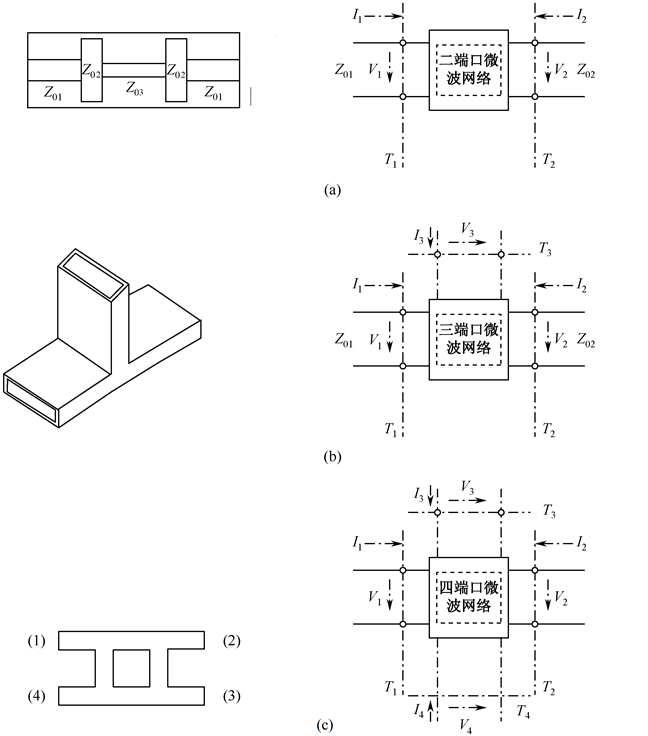
\includegraphics[width=6cm]{Cha5//fig5-4.png}
              \end{figure}
    \end{enumerate}
\end{frame}

\subsection{微波网络参量}
\begin{frame}{微波网络参量}
    \begin{enumerate}
        \item 微波网络的电路参量\\
              \begin{figure}
                  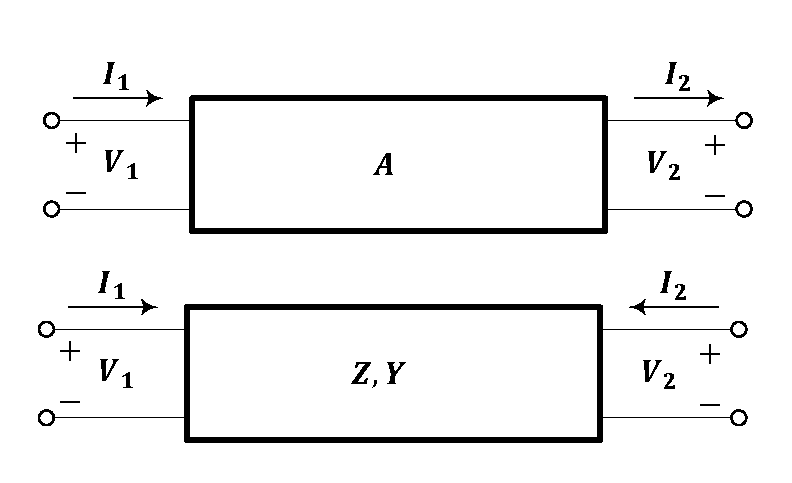
\includegraphics[width=7cm]{Cha5//fig5-5.pdf}
                  \caption{用$Z,Y和A$参数表示的二端口网络示意图}
              \end{figure}
    \end{enumerate}
\end{frame}

\begin{frame}{微波网络参量}
    \begin{enumerate}
        \item 微波网络的电路参量
              \begin{itemize}
                  \item 阻抗矩阵$[Z]$:反映电压、电流关系
              \end{itemize}
              \begin{figure}
                  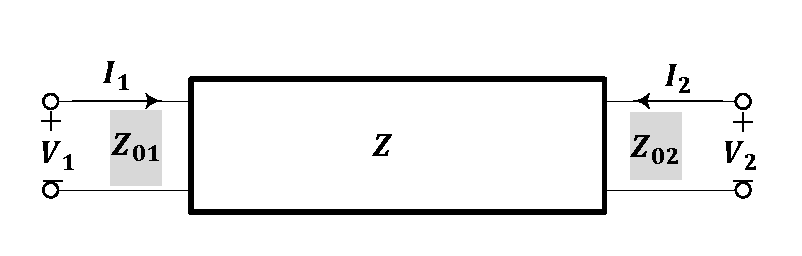
\includegraphics[width=7cm]{Cha5//fig5-6.pdf}
              \end{figure}
              \begin{gather}
                  \begin{bmatrix*}
                      V_1\\
                      V_2\\
                  \end{bmatrix*}
                  =
                  \begin{bmatrix*}
                      Z_{11} & Z_{12}\\
                      Z_{21} & Z_{22}\\
                  \end{bmatrix*}
                  \begin{bmatrix*}
                      I_1 \\
                      I_2 \\
                  \end{bmatrix*}\label{eqn5-1}\\
                  [V]=[Z][I]\label{eqn5-2}
              \end{gather}
    \end{enumerate}
\end{frame}

\begin{frame}{微波网络参量}
    \begin{enumerate}
        \item 微波网络的电路参量
              \begin{itemize}
                  \item 网络的“开路”参数:“自阻抗”和“转移阻抗”
              \end{itemize}
              \begin{gather*}
                  \begin{bmatrix*}
                      V_1\\
                      V_2\\
                  \end{bmatrix*}
                  =
                  \begin{bmatrix*}
                      Z_{11} & Z_{12}\\
                      Z_{21} & Z_{22}\\
                  \end{bmatrix*}
                  \begin{bmatrix*}
                      I_1 \\
                      I_2 \\
                  \end{bmatrix*}\\
                  \begin{matrix*}
                      V_1=Z_{11}\cdot I_1+Z_{12}\cdot I_2\\
                      V_2=Z_{21}\cdot I_1+Z_{22}\cdot I_2\\
                  \end{matrix*}
                  \qquad Z=\frac{V}{I}\\
                  \begin{matrix*}
                      Z_{11}=\dfrac{V_1}{I_1}|_{I_2=0} & Z_{21}=\dfrac{V_2}{I_1}|_{I_2=0} & 2端口开路 \\
                      Z_{22}=\dfrac{V_2}{I_2}|_{I_1=0} & Z_{12}=\dfrac{V_1}{I_2}|_{I_1=0} & 1端口开路 \\
                  \end{matrix*}
              \end{gather*}
    \end{enumerate}
\end{frame}

\begin{frame}{微波网络参量}
    \begin{enumerate}
        \item 微波网络的电路参量
              \begin{itemize}
                  \item 归一化阻抗矩阵$[z]$:用$Z_{01},Z_{02}$归一化
              \end{itemize}
              \begin{gather}
                  \begin{bmatrix*}
                      v_1\\
                      v_2\\
                  \end{bmatrix*}
                  =
                  \begin{bmatrix*}
                      \frac{1}{\sqrt{Z_{01}}} & 0\\
                      0 & \frac{1}{\sqrt{Z_{02}}}\\
                  \end{bmatrix*}
                  \begin{bmatrix*}
                      V_1 \\
                      V_2 \\
                  \end{bmatrix*}\label{eqn5-3}\\
                  \hspace*{\fill}
                  \begin{bmatrix*}
                      i_1\\
                      i_2\\
                  \end{bmatrix*}
                  =
                  \begin{bmatrix*}
                      \sqrt{Z_{01}} & 0\\
                      0 & \sqrt{Z_{02}}\\
                  \end{bmatrix*}
                  \begin{bmatrix*}
                      I_1 \\
                      I_2 \\
                  \end{bmatrix*}
                  \label{eqn5-4}
              \end{gather}
              根据式(\ref{eqn5-1})和式(\ref{eqn5-3}),(\ref{eqn5-4})有
              \begin{gather*}
                  \begin{bmatrix*}
                      \frac{1}{\sqrt{Z_{01}}} & 0\\
                      0 & \frac{1}{\sqrt{Z_{02}}}\\
                  \end{bmatrix*}^{-1}
                  \begin{bmatrix*}
                      v_1 \\
                      v_2 \\
                  \end{bmatrix*}
                  =
                  \begin{bmatrix*}
                      Z_{11} & Z_{12}\\
                      Z_{21} & Z_{22}\\
                  \end{bmatrix*}
                  \begin{bmatrix*}
                      \sqrt{Z_{01}} & 0\\
                      0 & \sqrt{Z_{02}}\\
                  \end{bmatrix*}^{-1}
                  \begin{bmatrix*}
                      i_1\\
                      i_2\\
                  \end{bmatrix*}
              \end{gather*}
    \end{enumerate}
\end{frame}

\begin{frame}{微波网络参量}
    \begin{enumerate}
        \item 微波网络的电路参量
              \begin{itemize}
                  \item 归一化阻抗矩阵$[z]$:用$Z_{01},Z_{02}$归一化
              \end{itemize}
              \begin{gather}
                  \begin{bmatrix*}
                      v_1 \\
                      v_2 \\
                  \end{bmatrix*}
                  =
                  \begin{bmatrix*}
                      \frac{1}{\sqrt{Z_{01}}} & 0\\
                      0 & \frac{1}{\sqrt{Z_{02}}}\\
                  \end{bmatrix*}
                  \begin{bmatrix*}
                      Z_{11} & Z_{12}\\
                      Z_{21} & Z_{22}\\
                  \end{bmatrix*}
                  \begin{bmatrix*}
                      \sqrt{Z_{01}} & 0\\
                      0 & \sqrt{Z_{02}}\\
                  \end{bmatrix*}^{-1}
                  \begin{bmatrix*}
                      i_1\\
                      i_2\\
                  \end{bmatrix*}\label{eqn5-5}\\
                  \Rightarrow
                  \begin{bmatrix*}
                      v_1 \\
                      v_2 \\
                  \end{bmatrix*}
                  =
                  \begin{bmatrix*}
                      \dfrac{Z_{11}}{Z_{01}} & \dfrac{Z_{12}}{\sqrt{Z_{01}\cdot Z_{02}}}\\
                      \dfrac{Z_{21}}{\sqrt{Z_{01}\cdot Z_{02}}} & \dfrac{Z_{22}}{Z_{02}}\\
                  \end{bmatrix*}
                  \begin{bmatrix*}
                      i_1 \\
                      i_2 \\
                  \end{bmatrix*}\label{eqn5-6}
                  \qquad
                  [v]=[z][i]
              \end{gather}
    \end{enumerate}
\end{frame}

\begin{frame}{微波网络参量}
    \begin{enumerate}
        \item 微波网络的电路参量
              \begin{table}
                  \caption{阻抗矩阵单元物理意义}
                  \footnotesize
                  \begin{tabular}{|c|c|c|}
                      \hline
                      \textbf{阻抗矩阵阵元}   & \textbf{计算公式}                            & \textbf{物理意义}             \\ \hline
                      $Z_{11}$ & $\dfrac{V_1}{I_1}\bigg\vert_{I_2=0}$ & 输出端口开路情况下的输入阻抗   \\ \hline
                      $Z_{12}$ & $\dfrac{V_1}{I_2}\bigg\vert_{I_1=0}$ & 输入端口开路情况下的反向传输阻抗 \\ \hline
                      $Z_{21}$ & $\dfrac{V_2}{I_1}\bigg\vert_{I_2=0}$ & 输出端口开路情况下的正向传输阻抗 \\ \hline
                      $Z_{22}$ & $\dfrac{V_2}{I_2}\bigg\vert_{I_1=0}$ & 输入端口开路情况下的输出阻抗   \\ \hline
                  \end{tabular}
              \end{table}
    \end{enumerate}
\end{frame}

\begin{frame}{微波网络参量}
    \begin{enumerate}
        \item 微波网络的电路参量
              \begin{itemize}
                  \item 导纳矩阵$[Y]$
                        \begin{figure}
                            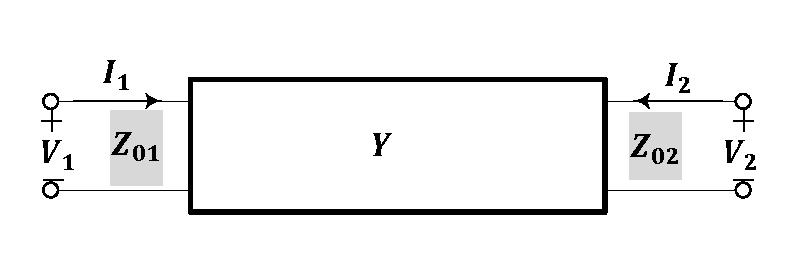
\includegraphics[width=8cm]{Cha5//fig5-7.pdf}
                        \end{figure}
                        \begin{gather*}
                            \begin{bmatrix*}
                                I_1\\
                                I_2\\
                            \end{bmatrix*}
                            =
                            \begin{bmatrix*}
                                Y_{11} & Y_{12}\\
                                Y_{21} & Y_{22}\\
                            \end{bmatrix*}
                            \begin{bmatrix*}
                                V_1 \\
                                V_2 \\
                            \end{bmatrix*}\\
                            [I]=[Y][V]
                        \end{gather*}
              \end{itemize}
    \end{enumerate}
\end{frame}

\begin{frame}{微波网络参量}
    \begin{enumerate}
        \item 微波网络的电路参量
              \begin{itemize}
                  \item 网络的“短路”参数:“自导纳”和“转移导纳”
                        \begin{gather*}
                            \begin{bmatrix*}
                                I_1\\
                                I_2\\
                            \end{bmatrix*}
                            =
                            \begin{bmatrix*}
                                Y_{11} & Y_{12}\\
                                Y_{21} & Y_{22}\\
                            \end{bmatrix*}
                            \begin{bmatrix*}
                                V_1 \\
                                V_2 \\
                            \end{bmatrix*}\\
                            Y_{ij}=\frac{I_i}{V_j}|_{V_k=0,k\neq j}
                        \end{gather*}
                        所有其他端口短路时,驱动端口$j$的电压为$V_j$时在端口$i$测得的短路电流来确定。
                        \begin{gather*}
                            [i]=[y][v] \qquad
                            [y]=
                            \begin{bmatrix*}
                                Y_{11}Z_{01} & Y_{12}\sqrt{Z_{01}Z_{02}} \\
                                Y_{21}\sqrt{Z_{01}Z_{02}} & Y_{22}Z_{02} \\
                            \end{bmatrix*}
                        \end{gather*}
              \end{itemize}
    \end{enumerate}
\end{frame}

\begin{frame}{微波网络参量}
    \begin{enumerate}
        \item 微波网络的电路参量
        \begin{table}
            \caption{导纳矩阵单元物理意义}
            \footnotesize
            \begin{tabular}{|c|c|c|}
                \hline
                \textbf{导纳矩阵阵元}   & \textbf{计算公式}                            & \textbf{物理意义}             \\ \hline
                $Y_{11}$ & $\dfrac{I_1}{V_1}\bigg\vert_{V_2=0}$ & 输出端口短路情况下的输入导纳   \\ \hline
                $Y_{12}$ & $\dfrac{I_1}{V_2}\bigg\vert_{V_1=0}$ & 输入端口短路路情况下的反向传输导纳 \\ \hline
                $Y_{21}$ & $\dfrac{I_2}{V_1}\bigg\vert_{V_2=0}$ & 输出端口短路情况下的正向传输导纳 \\ \hline
                $Y_{22}$ & $\dfrac{I_2}{V_2}\bigg\vert_{V_1=0}$ & 输入端口短路情况下的输出导纳   \\ \hline
            \end{tabular}
        \end{table}
    \end{enumerate}
\end{frame}

\begin{frame}{微波网络参量}
    \begin{enumerate}
        \item 微波网络的电路参量
        \begin{itemize}
            \item 转移矩阵$[A]$
            \begin{figure}
                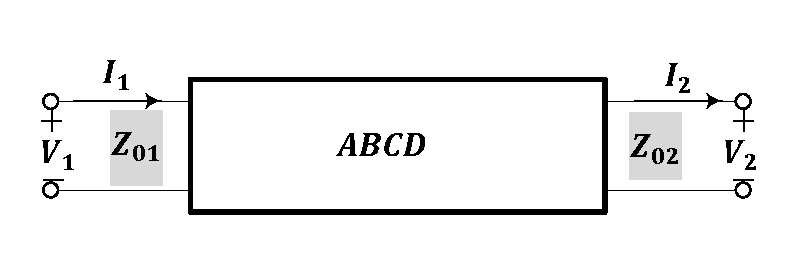
\includegraphics[width=8cm]{Cha5//fig5-8.pdf}
            \end{figure}
            \begin{gather*}
                \begin{bmatrix*}
                    V_1 \\
                    I_1 \\
                \end{bmatrix*}
                =
                \begin{bmatrix*}
                    A & B \\
                    C & D \\
                \end{bmatrix*}
                \begin{bmatrix*}
                    V_2 \\
                    I_2 \\
                \end{bmatrix*}\quad\rightarrow\quad
                \begin{cases}
                    V_1=A\cdot V_2+B\cdot I_2\\
                    I_1=C\cdot V_2+D\cdot I_2
                \end{cases}
            \end{gather*}
        \end{itemize}
    \end{enumerate}
\end{frame}

\begin{frame}{微波网络参量}
    \begin{enumerate}
        \item 微波网络的电路参量
    \end{enumerate}
\end{frame}

\begin{frame}{微波网络参量}
    \begin{enumerate}
        \item 微波网络的电路参量
    \end{enumerate}
\end{frame}

\subsection{微波网络参量的性质}
\begin{frame}{微波网络参量的性质}

\end{frame}

\subsection{二端口微波网络的工作特性参量}
\begin{frame}{二端口微波网络的工作特性参量}

\end{frame}

\subsection{微波网络的组合}
\begin{frame}{微波网络的组合}

\end{frame}

\subsection{二端口网络的等效电路}
\begin{frame}{二端口网络的等效电路}

\end{frame}

\subsection{信号流图分析及其应用}
\begin{frame}{信号流图分析及其应用}

\end{frame}

